\documentclass{article}

\usepackage[utf8x]{inputenc}
\usepackage[T1]{fontenc}
\usepackage[francais]{babel}
\usepackage{lmodern}
\usepackage{amsthm}
\usepackage{amsmath}
\usepackage{amssymb}
\usepackage{mathrsfs}
\usepackage{verbatim}
\usepackage{moreverb}
\usepackage[top=3cm, bottom=2cm, left=3cm, right=3cm]{geometry}
\usepackage{graphicx}
\usepackage{hyperref}
\usepackage{minted}
\usepackage{soul}
\usepackage{longtable}

\setlongtables

\hypersetup{colorlinks=true, linkcolor=red}

\author{Conrad \bsc{Hillairet} et Alexandre \bsc{Vieira}}
\title{Mini-projet : \\ \Large{JAVA}}
\date{\today}

\begin{document}
\maketitle

\setcounter{tocdepth}{4}
\tableofcontents
\newpage

\section*{Introduction}
Le but de notre projet est de concevoir un logiciel permettant de jouer à ce que nous appelons le jeu des drapeaux.

\bigskip
Le but de ce jeu est de reconnaître les drapeaux qui sont affichés à l'écran dans un temps limité. Chaque bonne réponse rapporte un point, qui sont comptabilisé. Nous avions donc plusieurs objectifs :
\begin{itemize}
	\item Concevoir une interface graphique
	\item A partir de celle-ci, pouvoir communiquer avec l'utilisateur
	\item Arriver à utiliser différentes ressources extérieures (images, compteur de temps, etc)
\end{itemize}

\bigskip
Ce projet utilisera plusieurs notions vu en cours, telle que les threads, les systèmes d'entrées-sorties et bien sûr, plus basiquement, les classes et les méthodes associées. Il utilise également beaucoup de notions qui n'ont pas encore été abordées, telle que les interfaces graphiques ou encore les patterns (MVC dans notre cas).

\begin{center}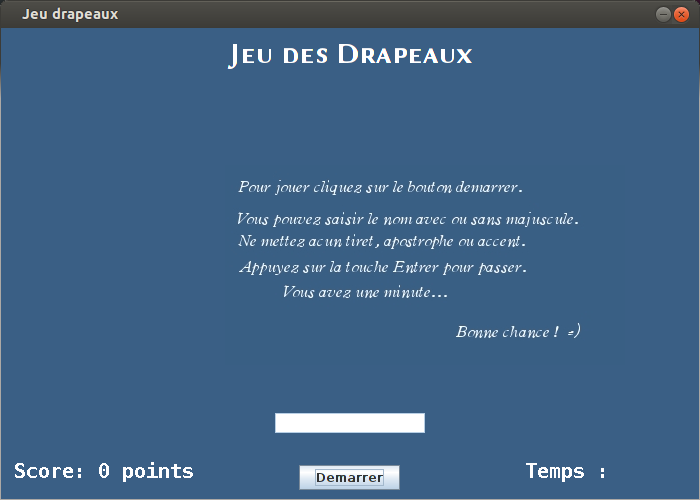
\includegraphics[scale=0.5]{intro.png}\end{center}

\newpage
\section{Présentation du projet : UML}
\subsection{BPM}
\begin{center}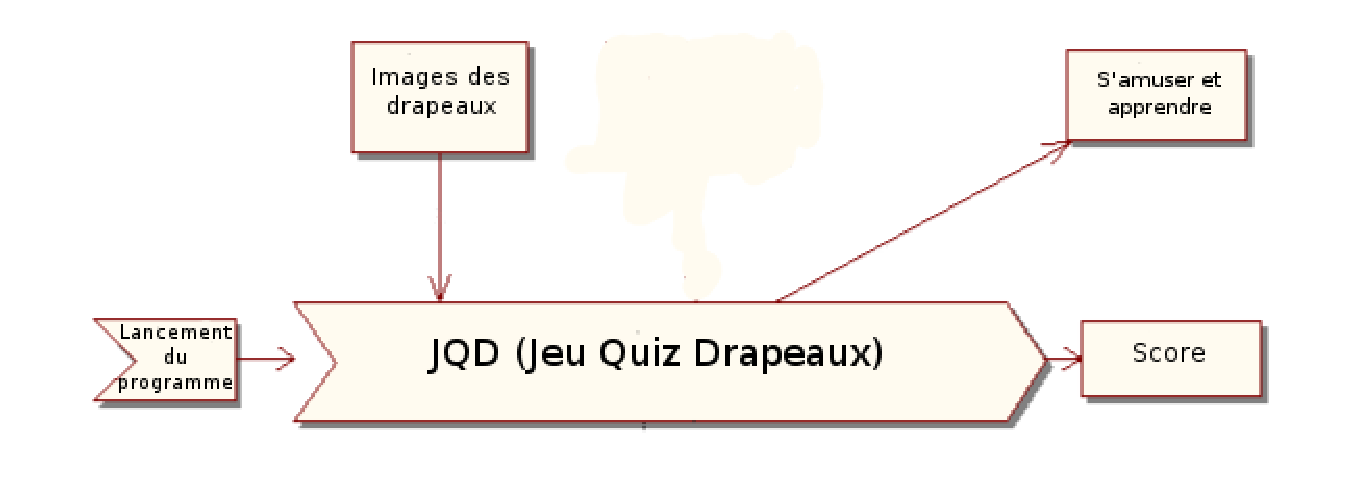
\includegraphics[scale=0.7]{BPM.eps}\end{center}

\subsection{Le pattern MVC}
Les Patterns, ou en français Patrons, sont des modèles de construction des programmes. Certains d'entre eux sont réputés pour apporter une certaine cohérence, robustesse et réutilisabilité, tout ce qu'on demande à un bon programme.\\
Nous avons ici utilisé le pattern MVC, pour Modèle-Vue-Contrôleur. Expliqué par un schéma, il s'articule dans notre projet ainsi :

\begin{center}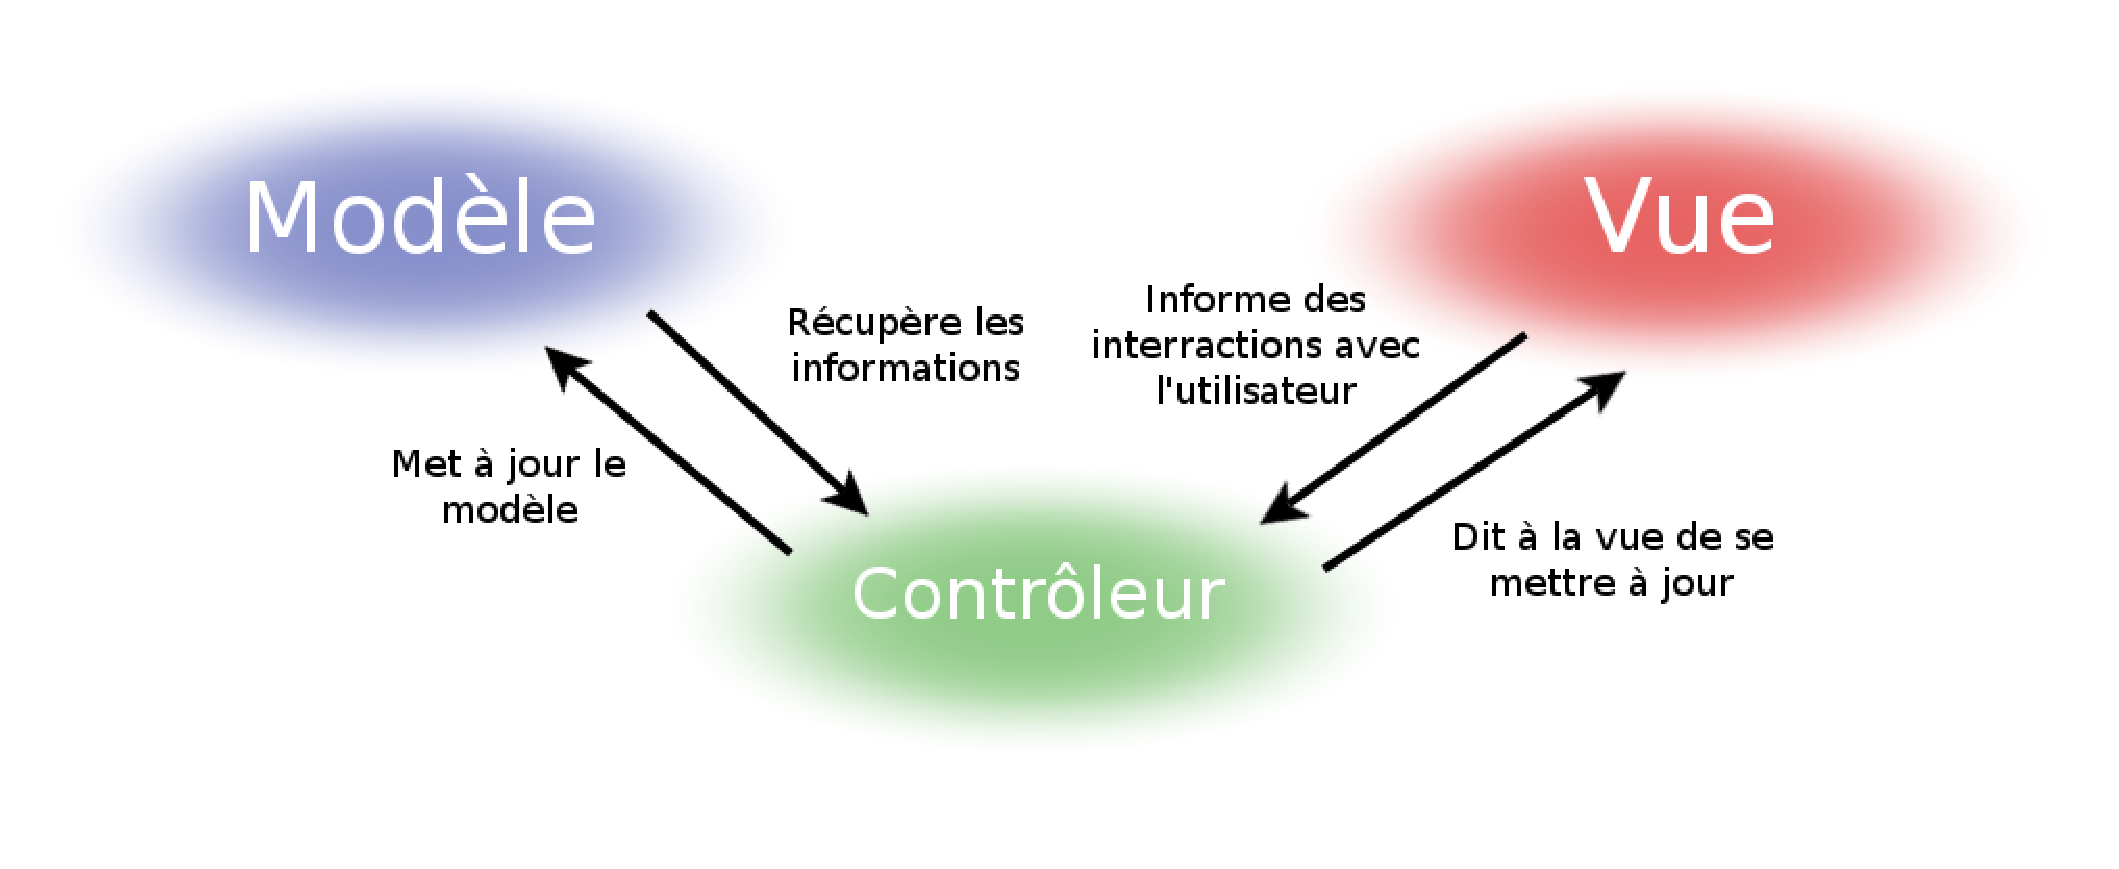
\includegraphics[scale=0.5]{MVC.eps}\end{center}

La plupart de nos explications et nos codes seront présentés organisés selon ces trois parties.

\subsection{Présentation des classes}
\subsubsection{Partie Vue}
\begin{center}
\begin{tabular}{|c|}
	\hline
	DessinDrapeau\\
	\hline
	- String chemin\\
	\hline
	+ DessinDrapeau()\\
	+ paintComponent(Graphics g)\\
	+ setChemin(String nouveauChemin)\\
	\hline
\end{tabular}
\hspace{2cm} \begin{tabular}{|c|}
	 \hline
	 DessinScore\\
	 \hline
	 + int score\\
	 \hline
	 + dessinScore()\\
	 + paintComponent(Graphics g)\\
	 + setScore(int nouveauScore)\\
	 \hline
\end{tabular}

\bigskip
\begin{tabular}{|c|}
	\hline
	DessinTemps\\
	\hline
	- String compteur\\
	\hline
	+ DessinTemps()\\
	+ paintComponent(Graphics g)\\
	+ setCompteur(String nouveauTemps)\\
	\hline
\end{tabular}\\
\begin{longtable}{|c|}
	\hline
	VueJQD\\
	\hline
	  //-Parametres de la fenetre\\
	  - String titre\\
	  - int largeur\\
	  - int hauteur\\
	  - boolean demarre\\
	  + DessinDrapeau dessinDrapeau\\
	  + DessinScore dessinScore\\
	  + DessinTemps dessinTemps\\
	  \\
	  //-Zones de la fenetre\\
	  //--Le conteneur principal\\
	  - JPanel container\\
	  \\
	  //--Le nom du jeu\\
	  + JLabel enTete\\
	  \\
	  //--La zone d'affichage du drapeau\\
	  + JPanel zoneImage\\
	  \\
	  //--La zone de reponse\\
	  + JPanel zoneReponse\\
	  \\
	  //---La zone de saisie de la reponse\\
	  + JTextField zoneSaisieReponse\\
	  \\
	  //--La zone de score, de temps et pour lancer le jeu\\
	  + JPanel piedDePage\\
	  \\
	  //---Le bouton demarrer\\
	  + JButton boutonDemarrer\\
	  \\
	  //--La zone de notification du nom du pays\\
	  + JLabel zoneNotifPays\\
	  \\
	  //Le controleur\\
	  + ControlerJQD controler\\
	\hline
	//Constructeurs\\
	+ VueJQD(ControlerJQD ctrl)\\
	\\
	//Accesseurs\\
	+ getString() : String\\
	+ getDemarre() : boolean\\
	+ setDemarre()\\
	+ setEnabledSaisieReponse(boolean bool)\\
	+ setScoreDessinScore(int i)\\
	+ setCompteurDessinTemps(String str)\\
	+ setCheminDessinDrapeau(String c)\\
	+ setEnabledBoutonDemarrer(boolean bool)\\
	+ setForegroundZoneNotifPays(Color col)\\
	+ setTextZoneNotifPays(String str)\\
	\\
	//Repaint\\
	+ repaintDessinScore()\\
	+ repaintDessinScore()\\
	+ repaintDessinDrapeau()\\
	+ repaintZoneNotifPays()\\
	\\
	//Autres méthodes\\
	+ iniJeu()\\
	\hline
\end{longtable}
\end{center}

\subsubsection{Partie Modèle}
\begin{center}
\begin{tabular}{|c|}
	\hline
	Drapeau\\
	\hline
	String nom\\
	String chemin\\
	\hline
	+ Drapeau()\\
	+ Drapeau(String nm, String chmn)\\
	+ getNom() : String\\
	+ getChemin() : String\\
	\hline
\end{tabular}
\begin{tabular}{|c|}
	\hline
	ListeDeDrapeaux\\
	\hline
	- ArrayList<Drapeau> listeDrapeau\\
	\hline
	+ ListeDeDrapeaux(String[] listePays, String[] listeChemin)\\
	+ getDrapeau(int i) : Drapeau\\
	\hline
\end{tabular}
\begin{tabular}{|c|}
	\hline
	GenerateurDrapeaux\\
	\hline
	- ListeDeDrapeaux listeDrap\\
	- Drapeau drapeauCourant\\
	- String[] listeNom\\
	- String[] listeChemin \\
	- GenerateurNbAleatoire generAlea\\
	\hline
	+ GenerateurDrapeaux()\\
	+ getDrapeauCourant() : Drapeau\\
	+ changerDrapeau()\\
	\hline
\end{tabular}
\hspace{2cm} \begin{tabular}{|c|}
	\hline
	GenerateurNbAleatoire\\
	\hline
	- int borneMin, borneSup\\
	\hline
	+ getBorneMin() : int\\
	+ getBorneSup() : int\\
	+ setBorneMin(int inf)\\
	+ setBorneSup(int max)\\
	+ genererNb() : int\\
	\hline
\end{tabular}
\begin{tabular}{|c|}
	\hline
	CompteurTemps\\
	\hline
	- long temps\\
	- long tempsMax\\
	- boolean statut\\
	\hline
	+ CompteurTemps(long t)\\
	+ getTemps() : long \\
	+ getStatut() : boolean \\
	+ setStatut(boolean b)\\
	+ run()\\
	+ toString() : String\\
	\hline
\end{tabular}
\hspace{2cm}\begin{tabular}{|c|}
	\hline
	Score\\
	\hline
	- int scorePartie\\
	\hline
	+ Score()\\
	+ getScore() : int\\
	+ setScore(int i) \\
	+ incrementerScore()\\
	+ remettreAZero()\\
	\hline
\end{tabular}
\begin{longtable}{|c|}
	\hline
	ModelJQD\\
	\hline
	\# CompteurTemps unCompteurTemps\\
	\# GenerateurDrapeaux generDrap\\
	\# Score unScore\\
	\hline
	//Accesseurs\\
	\# GenerateurDrapeaux getGenerateurDrapeaux()\\
	+ getDrapeauCourant() : Drapeau \\
	+ getScore() : int\\
	+ getCompteurTemps() : CompteurTemps \\
	+ getCheminDrapeauCourant() : String \\
	+ getNomDrapeauCourant() : String\\
	+ setMaxCompteurTemps(long t)\\
	+ setScore(int i)\\
	\\
	//Méthodes\\
	+ iniJeu()\\
	+ lancerCompteurTemps()\\
	+ scorePlusUn()\\
	+ changeDrapeauCourant()\\
	\hline
\end{longtable}

\end{center}

\subsubsection{Partie Contrôleur}
\begin{tabular}{|c|}
	\hline
	ControlerJQD\\
	\hline
	ModelJQD model\\
	VueJQD fenetre\\
	Actualiseur actualiseur\\
	\hline
	+ addFenetre(vueJQD f)\\
	+ demarrer()\\
	+ verif(String saisie)\\
	+ actualiser()\\
	\hline
\end{tabular}
\hspace{2cm} \begin{tabular}{|c|}
	 \hline
	 Actualiseur\\
	 \hline
	 VueJQD fenetre\\
	 ModelJQD model\\
	 \hline
	 + Actualiseur(VueJQD f, ModelJQD m)\\
	 + run()\\
	 \hline
 \end{tabular}

\subsubsection{Diagramme de classes}
\begin{center}
	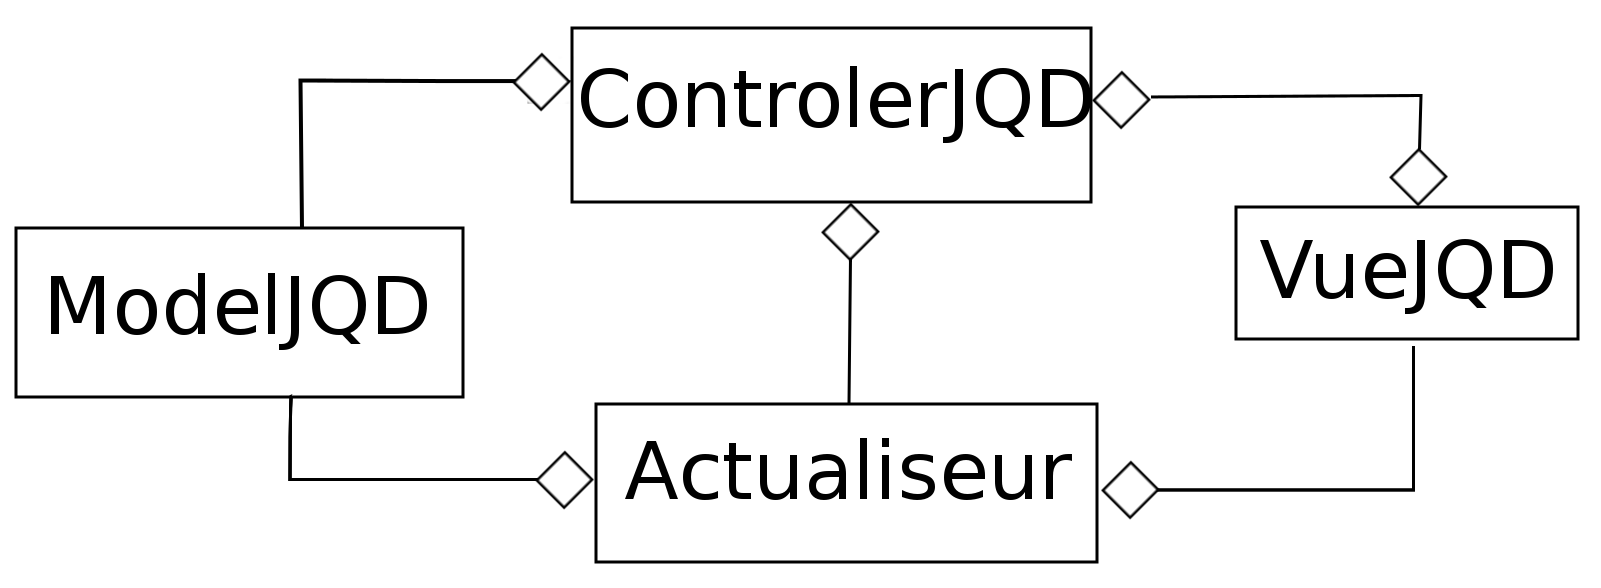
\includegraphics[scale=0.25]{diagClasse1.png}\\
	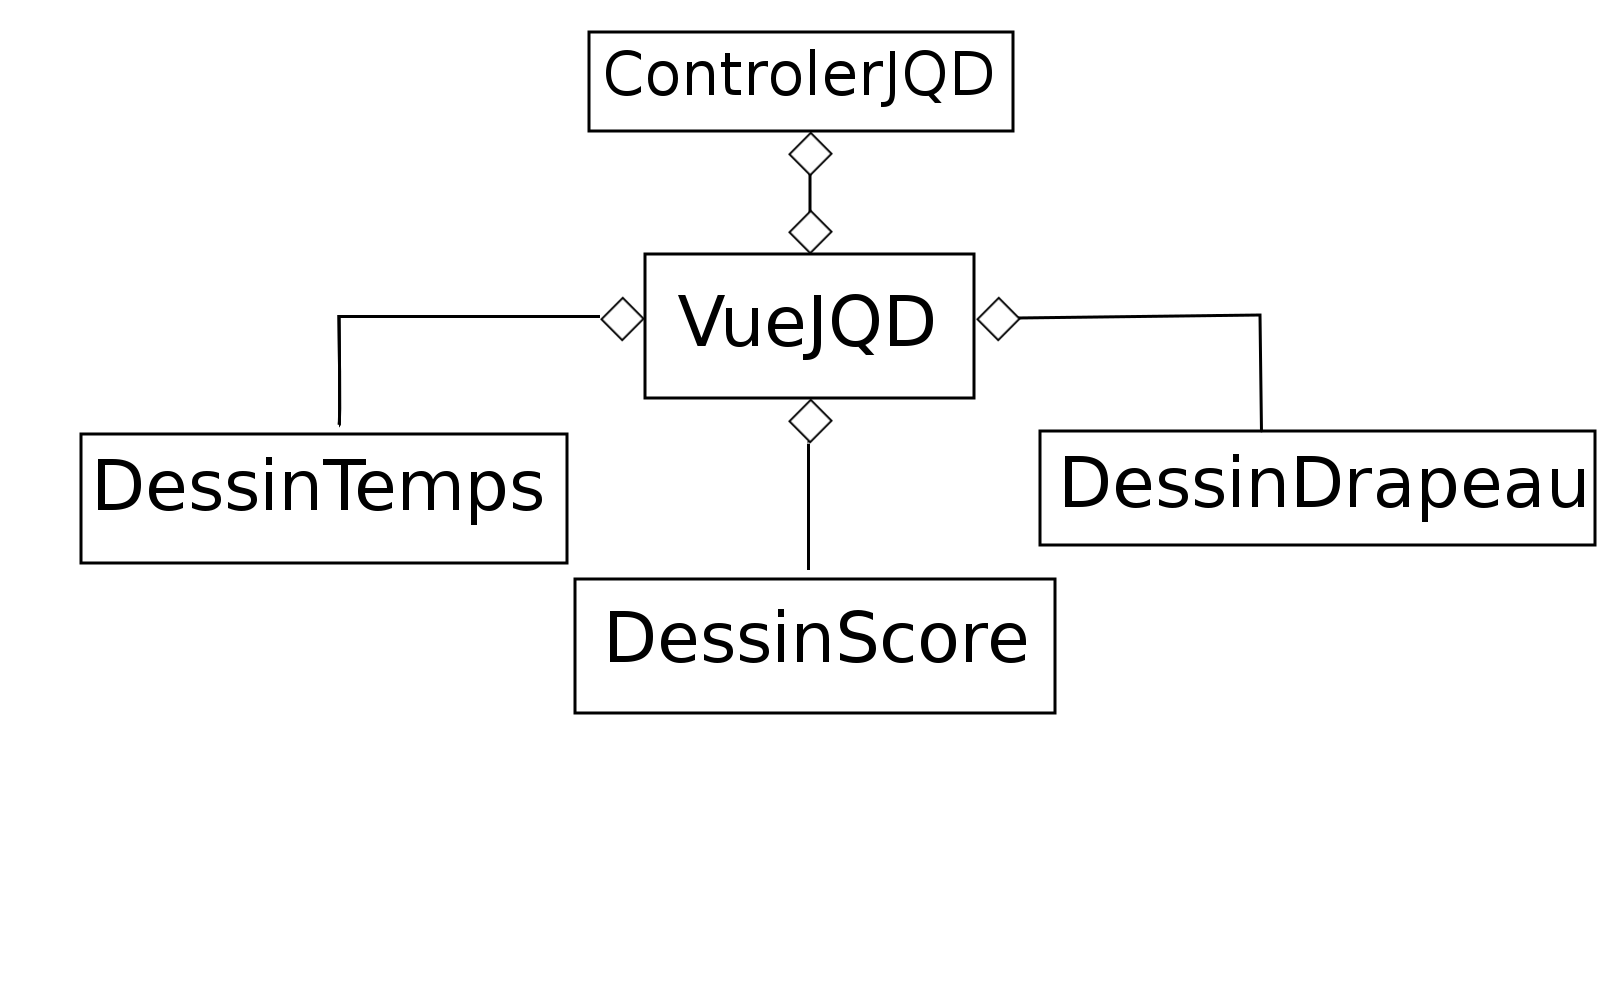
\includegraphics[scale=0.3]{diagClasse2.png}\\
	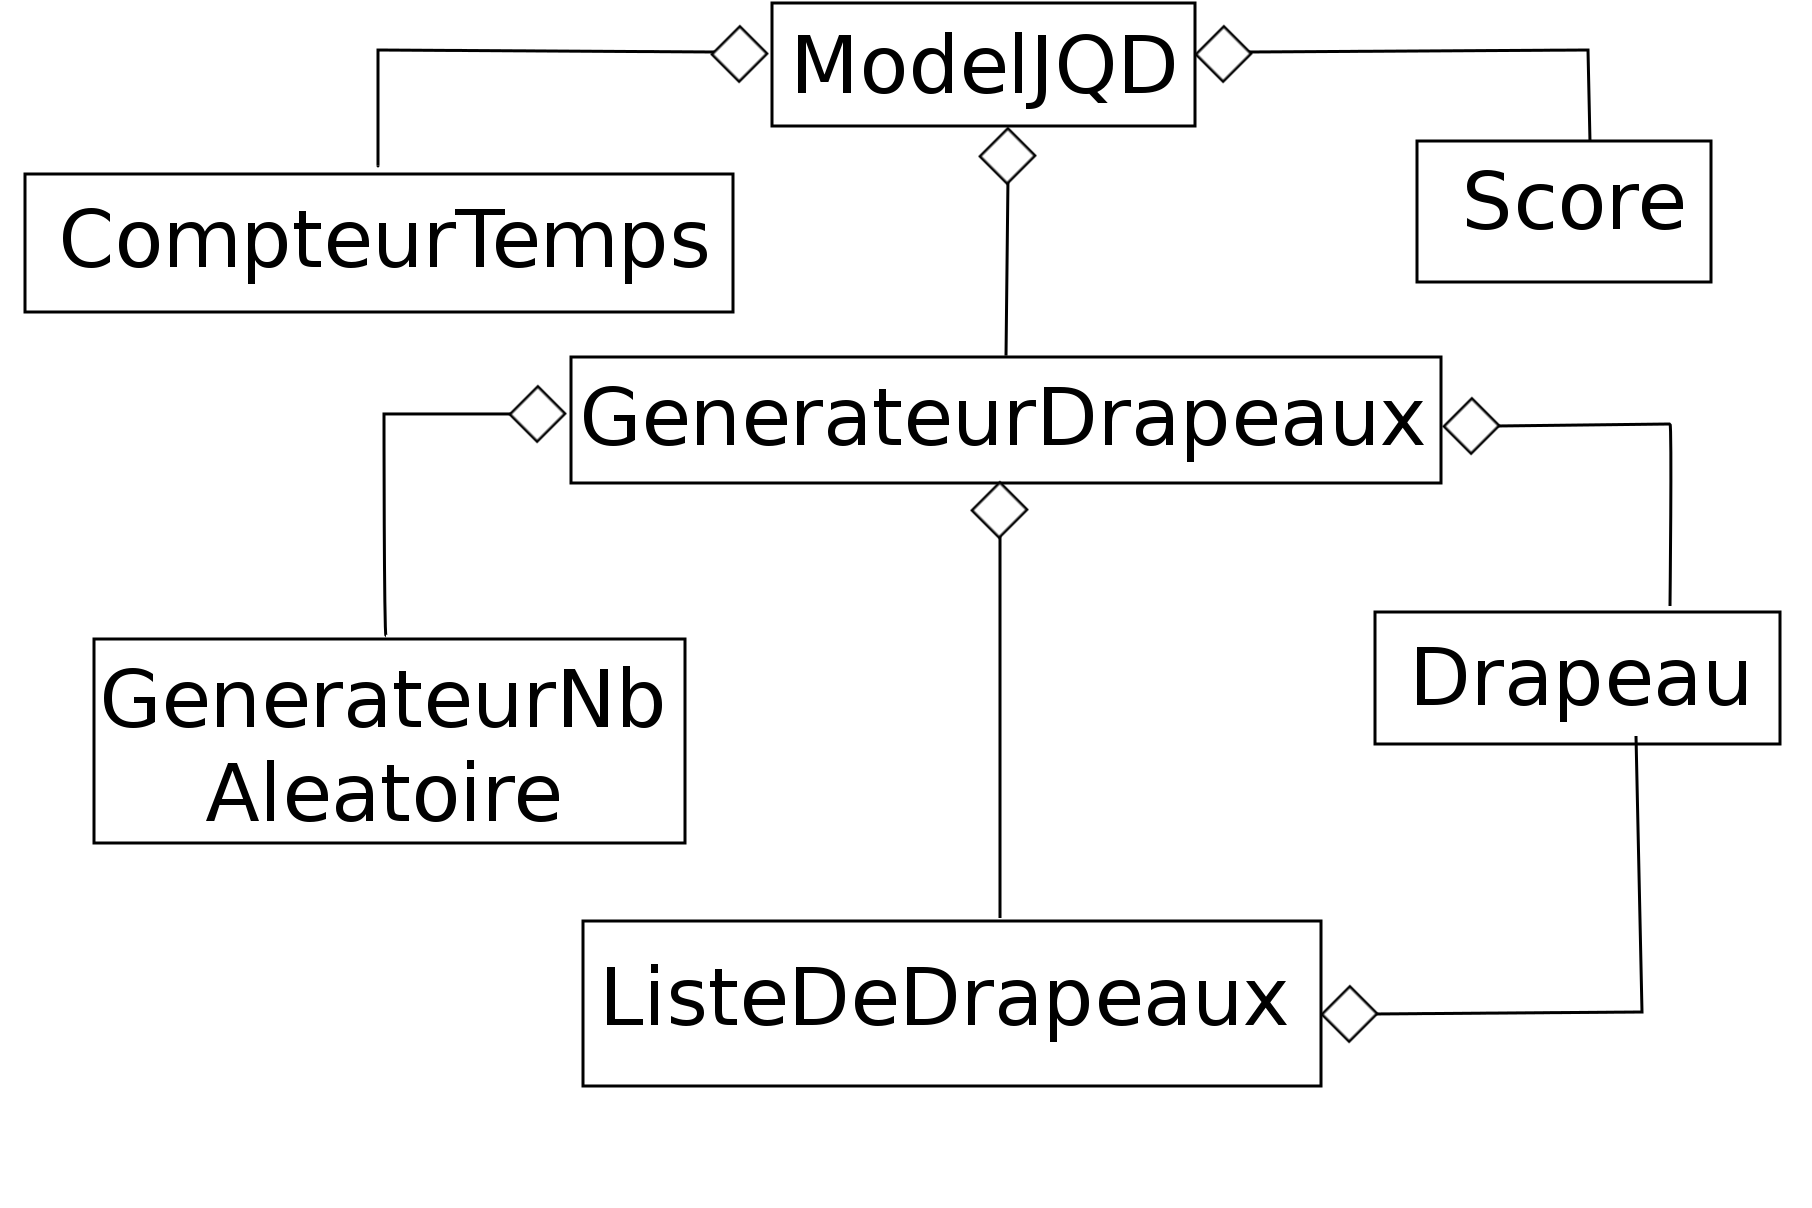
\includegraphics[scale=0.25]{diagClasse3.png}
\end{center}

\subsubsection{Diagramme de séquence}
\begin{center}
%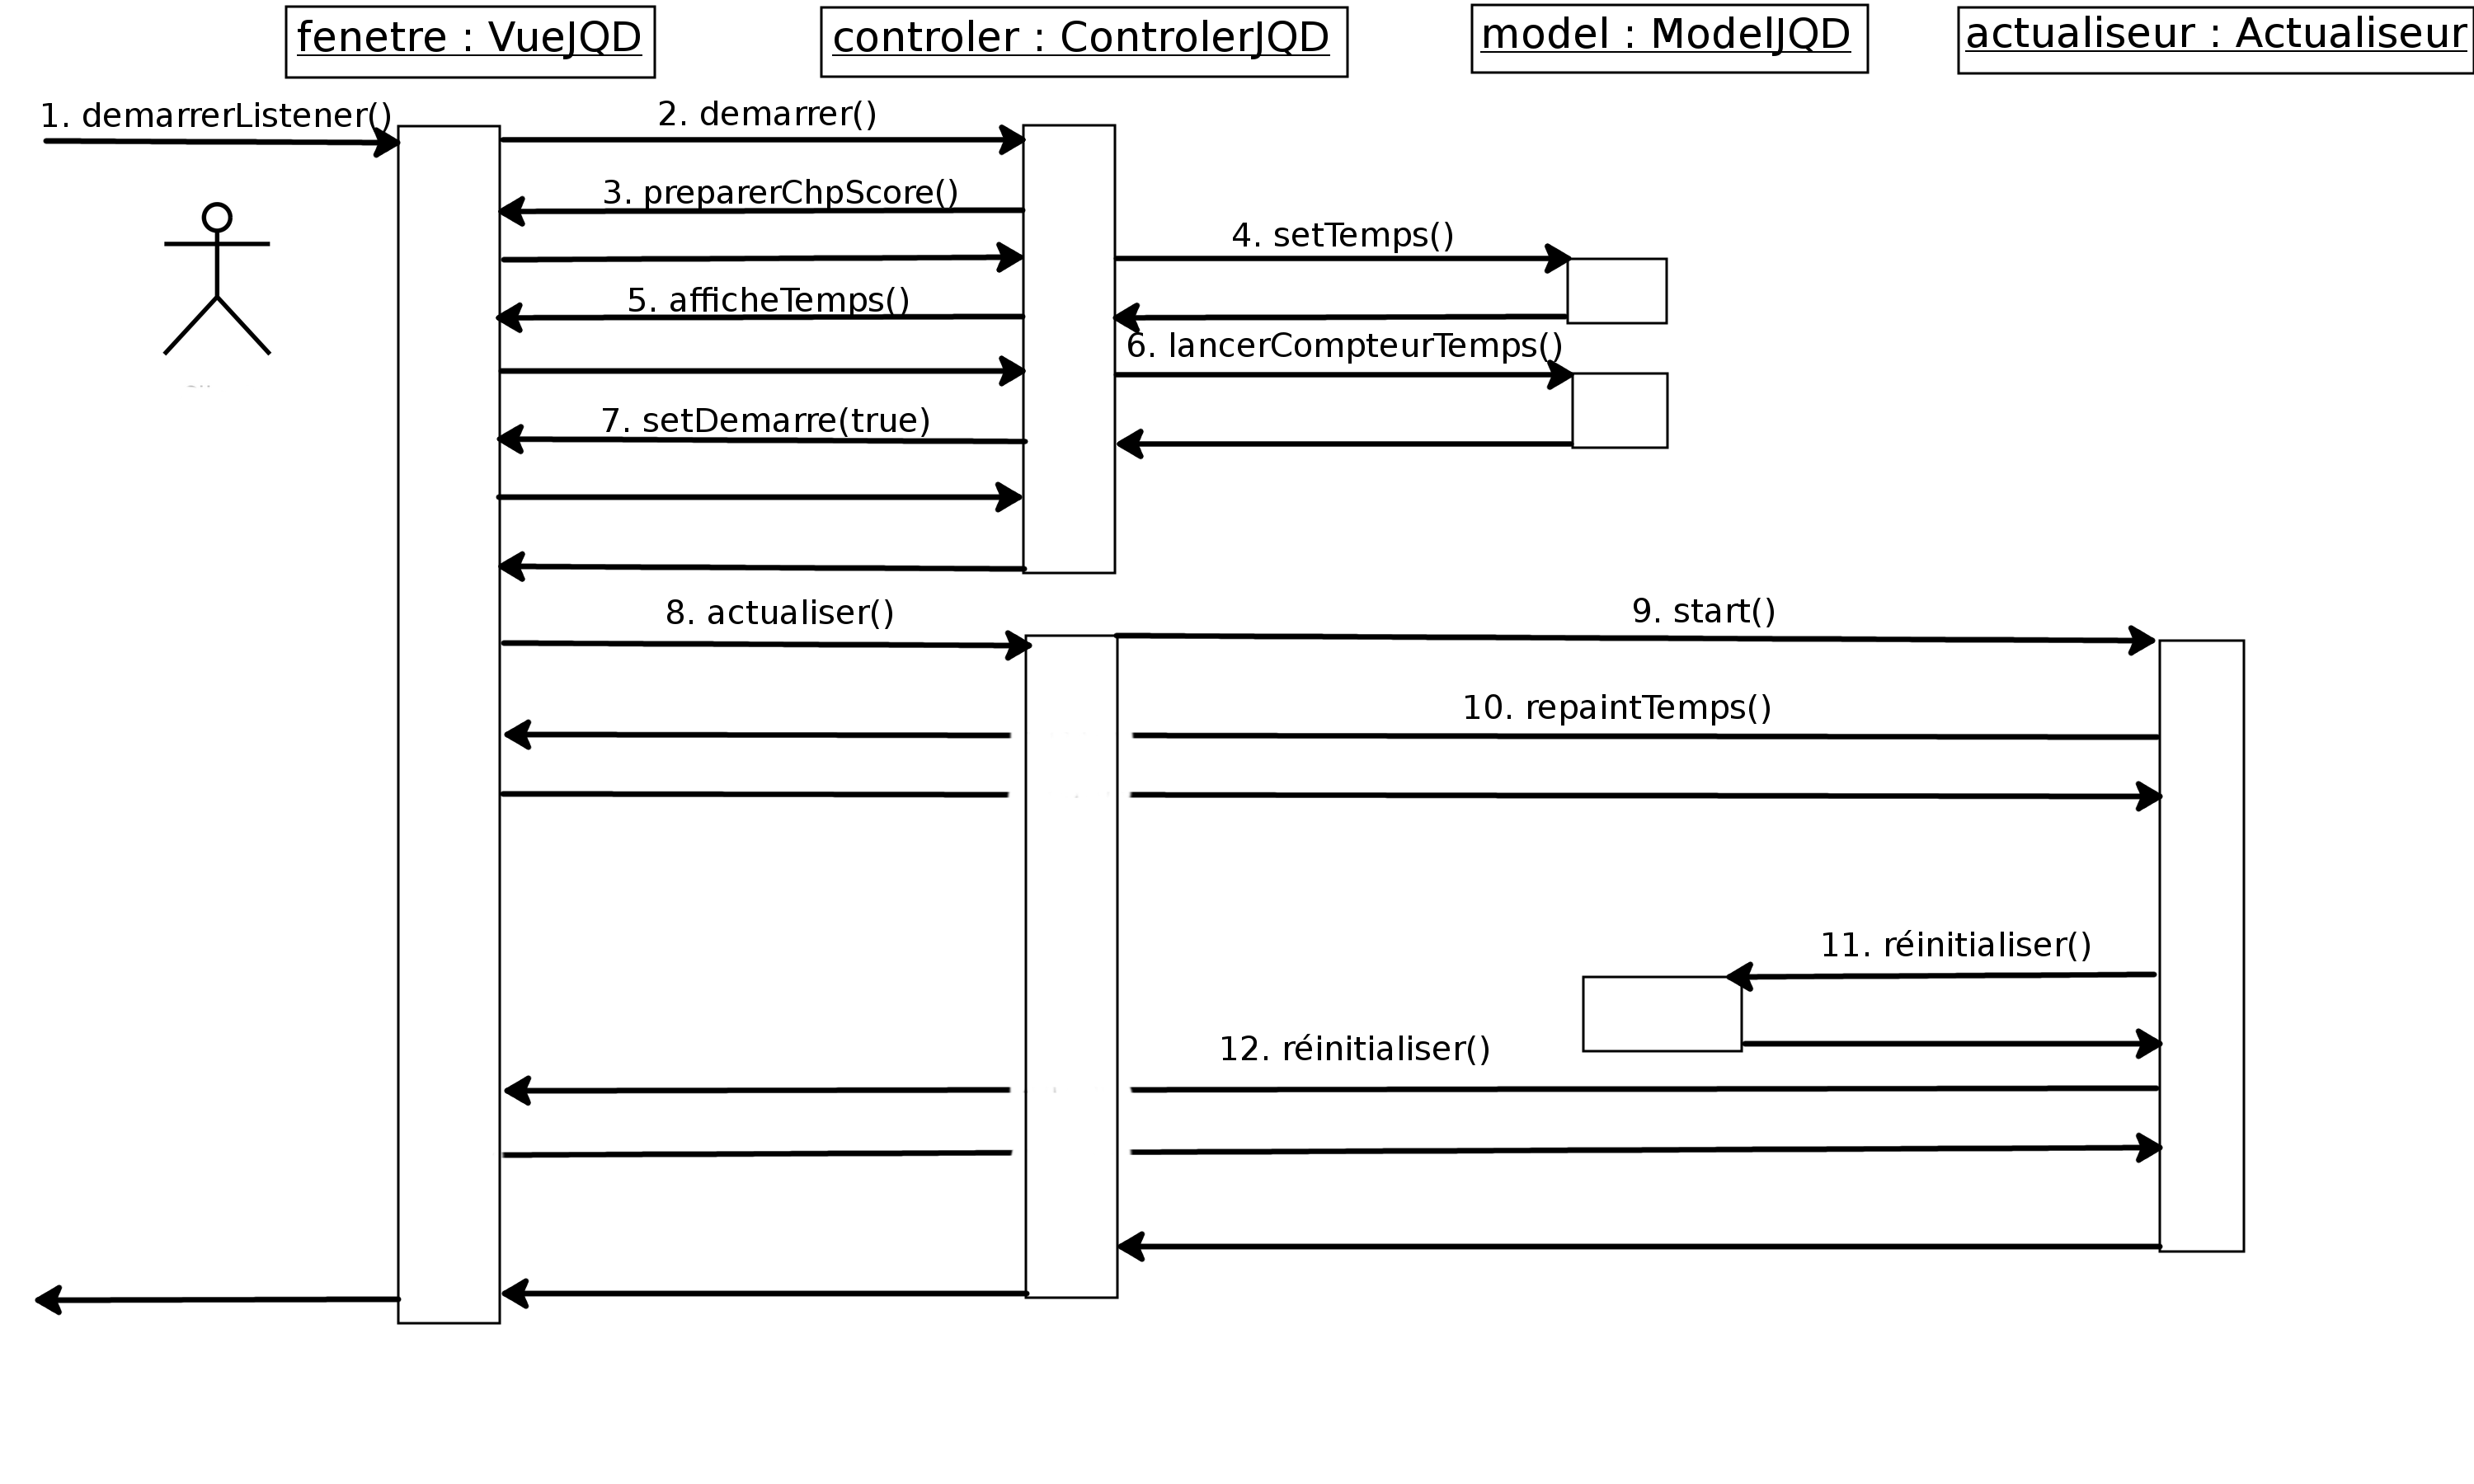
\includegraphics[scale=0.22,angle=-90]{diagMess.png}
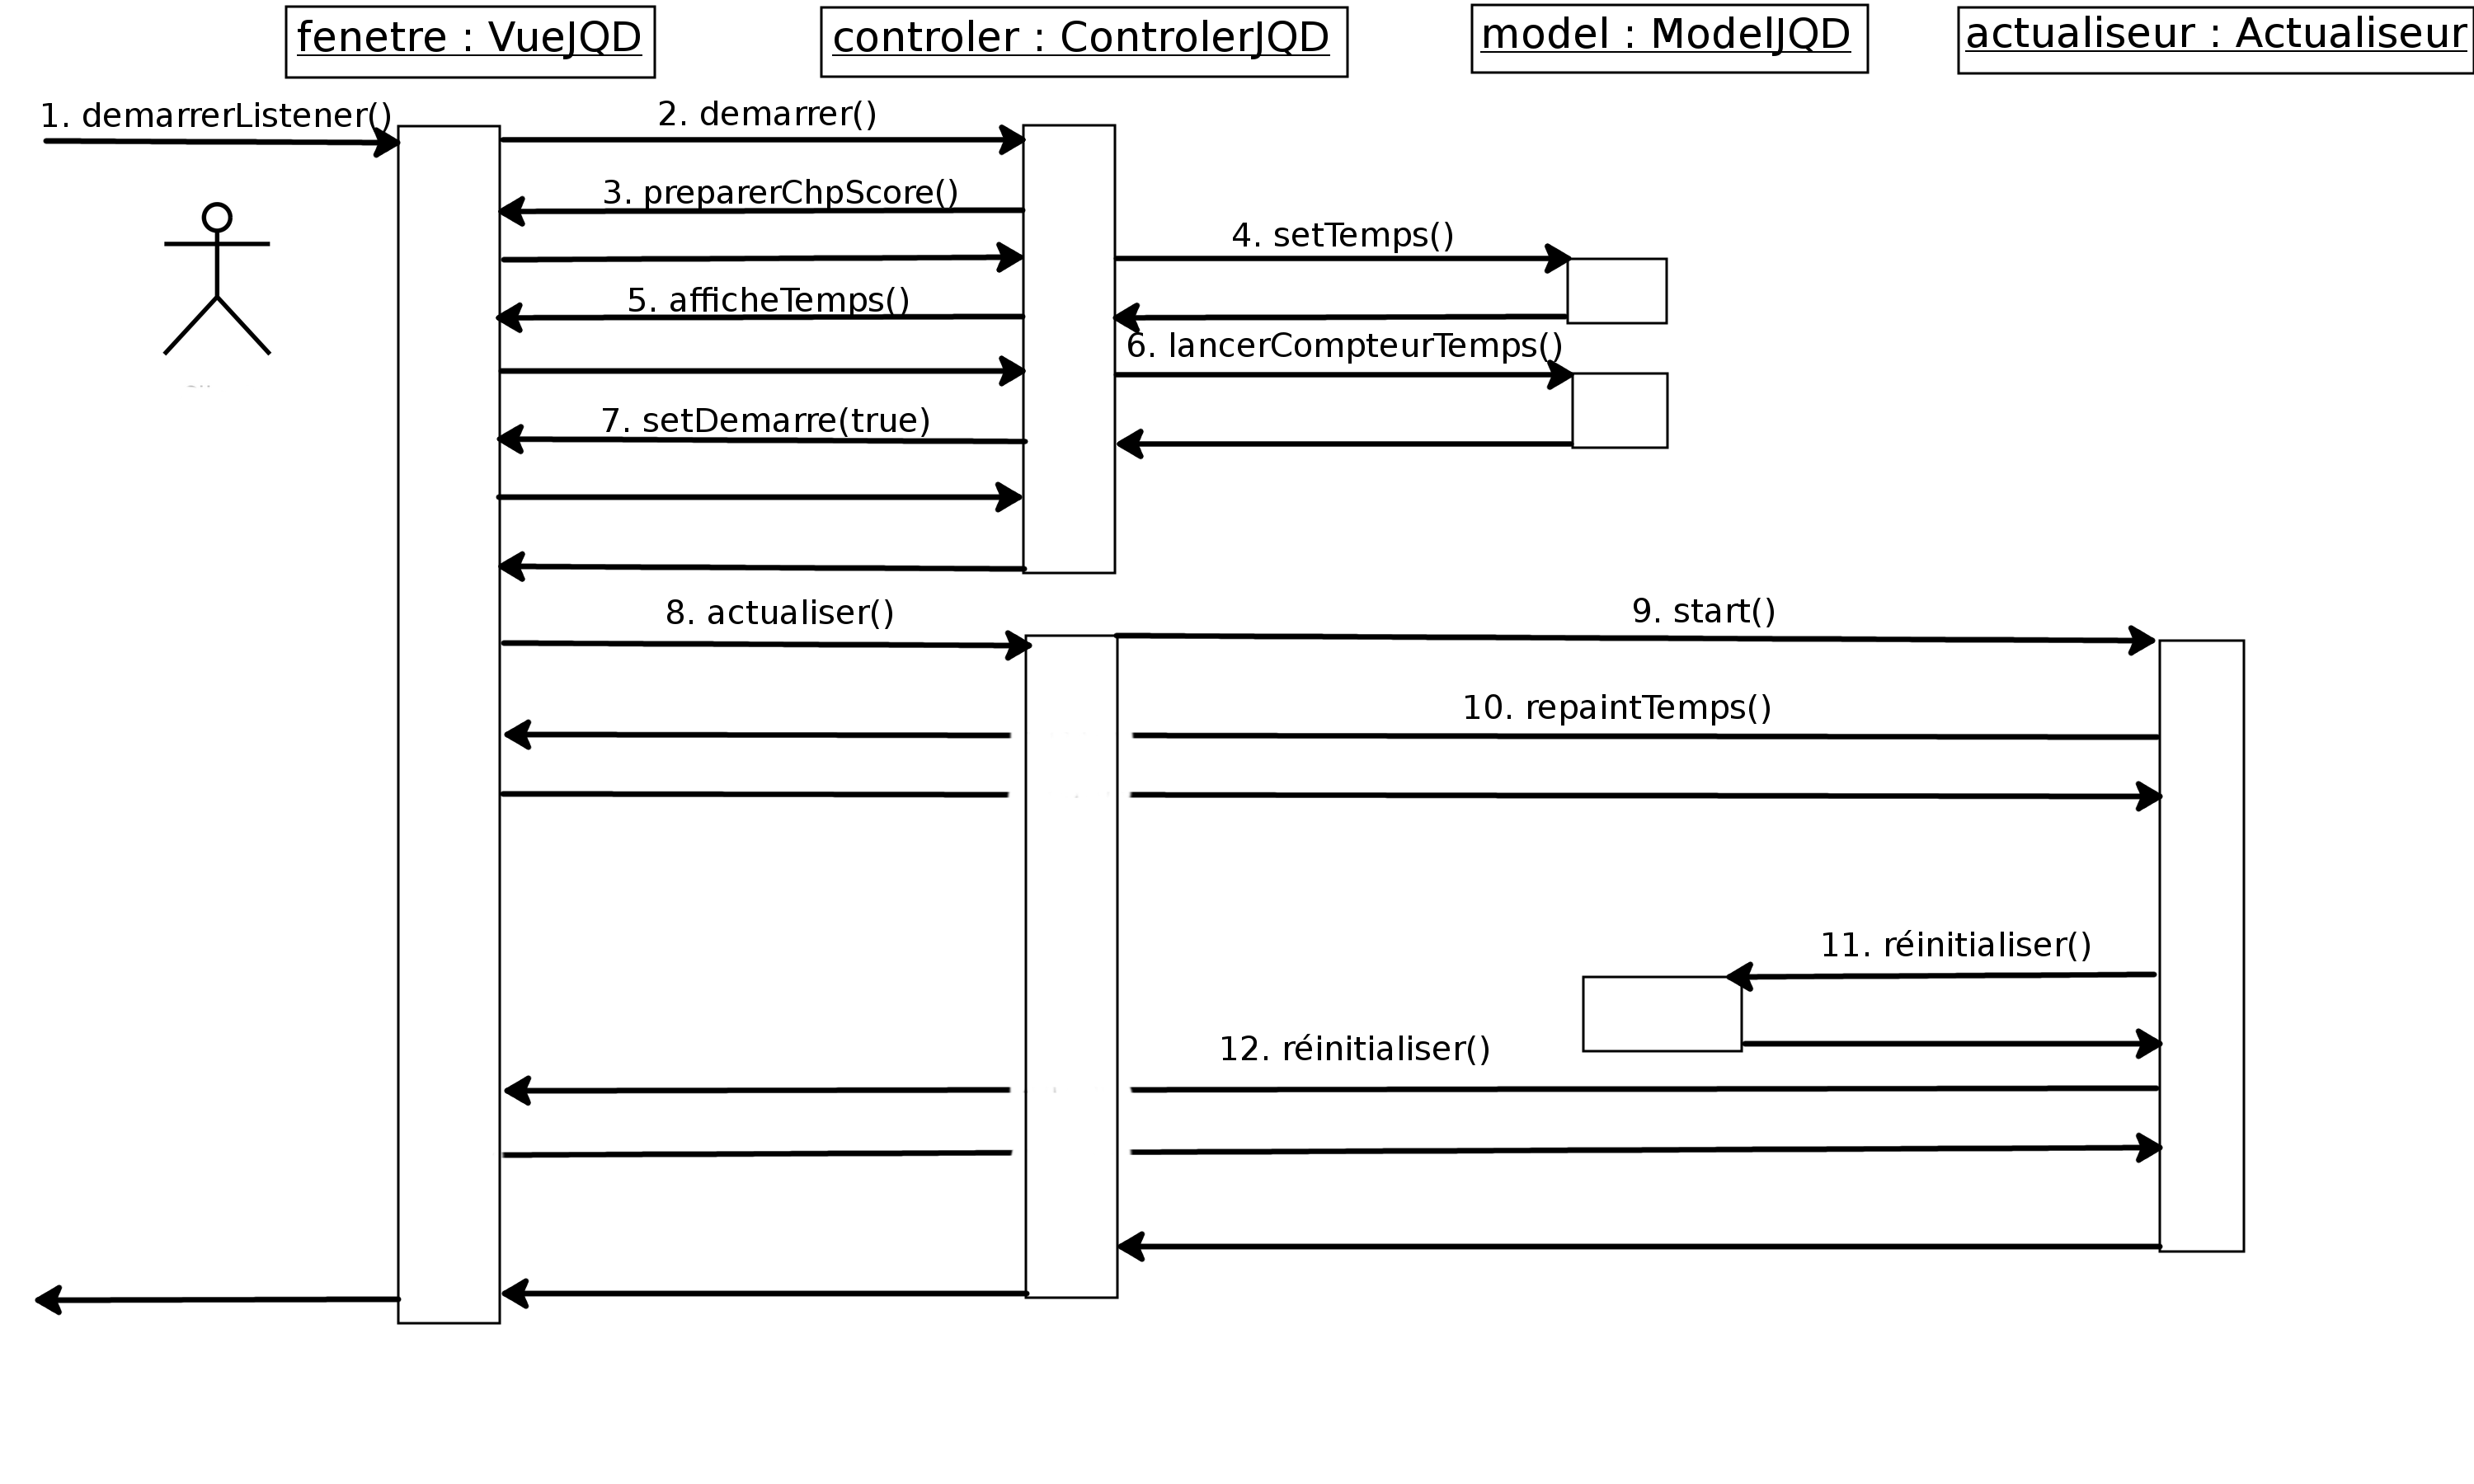
\includegraphics[scale=0.17]{diagMess.png}
\end{center}

\newpage
\section{Codes}
\subsection{Partie Vue}
\inputminted[frame=single]{java}{../encapsulation/DessinTemps.java}
\begin{center} \texttt{DessinTemps.java} \end{center}
\inputminted[frame=single]{java}{../encapsulation/DessinScore.java}
\begin{center} \texttt{DessinScore.java} \end{center}
\inputminted[frame=single]{java}{../encapsulation/DessinDrapeau.java}
\begin{center} \texttt{DessinDrapeau.java} \end{center}
\inputminted[frame=single]{java}{../encapsulation/VueJQD.java}
\begin{center} \texttt{VueJQD.java} \end{center}

\subsection{Partie Model}
\inputminted[frame=single]{java}{../encapsulation/Drapeau.java}
\begin{center} \texttt{Drapeau.java} \end{center}
\inputminted[frame=single]{java}{../encapsulation/ListeDeDrapeaux.java}
\begin{center} \texttt{ListeDeDrapeaux.java} \end{center}
	\begin{minted}[frame=single]{java}
public class GenerateurDrapeaux{
	private ListeDeDrapeaux listeDrap;
	private Drapeau drapeauCourant;
	private String[] listeNom={
"Afghanistan",
"Afrique du sud",
"Argentine",
...
};
	private String[] listeChemin={
"afghanistan.png",
"afrique_du_sud.png",
"argentine.png",
...
        };

	private GenerateurNbAleatoire generAlea=new GenerateurNbAleatoire(0,listeNom.length);

	public GenerateurDrapeaux(){
		listeDrap=new ListeDeDrapeaux(listeNom, listeChemin);
		drapeauCourant=listeDrap.getDrapeau(generAlea.genererNb());
	}

	public Drapeau getDrapeauCourant(){
		return drapeauCourant;
	}

	public void changerDrapeau(){
		drapeauCourant=listeDrap.getDrapeau(generAlea.genererNb());
	}
}
\end{minted}

\begin{center} \texttt{GenerateurDrapeaux.java} \end{center}
\inputminted[frame=single]{java}{../encapsulation/GenerateurNbAleatoire.java}
\begin{center} \texttt{GenerateurNbAleatoire.java} \end{center}
\inputminted[frame=single]{java}{../encapsulation/CompteurTemps.java}
\begin{center} \texttt{CompteurTemps.java} \end{center}
\inputminted[frame=single]{java}{../encapsulation/Score.java}
\begin{center} \texttt{Score.java} \end{center}
\inputminted[frame=single]{java}{../encapsulation/ModelJQD.java}
\begin{center} \texttt{ModelJQD.java} \end{center}

\subsection{Partie Controler}
\inputminted[frame=single]{java}{../encapsulation/Actualiseur.java}
\begin{center} \texttt{Actualiseur.java} \end{center}
\inputminted[frame=single]{java}{../encapsulation/ControlerJQD.java}
\begin{center} \texttt{Controler.java} \end{center}

\subsection{Main}
\inputminted[frame=single]{java}{../encapsulation/JQD.java}
\begin{center} \texttt{JQD.java} \end{center}

\newpage
\section{Captures d'écran}
\begin{center}
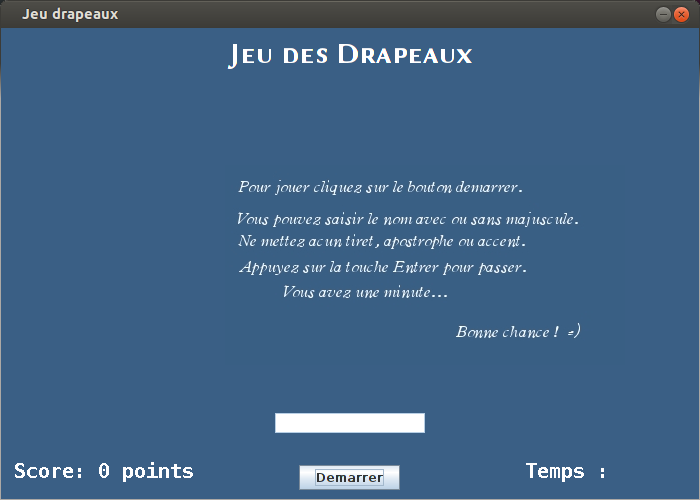
\includegraphics[scale=0.5]{intro.png}\\
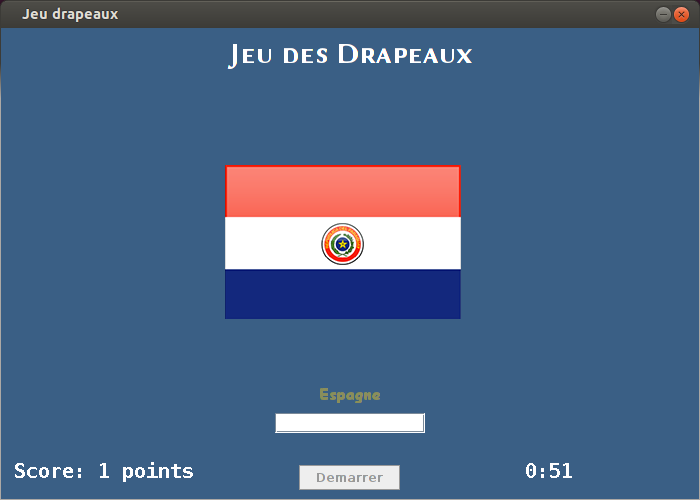
\includegraphics[scale=0.5]{capture1.png}\\
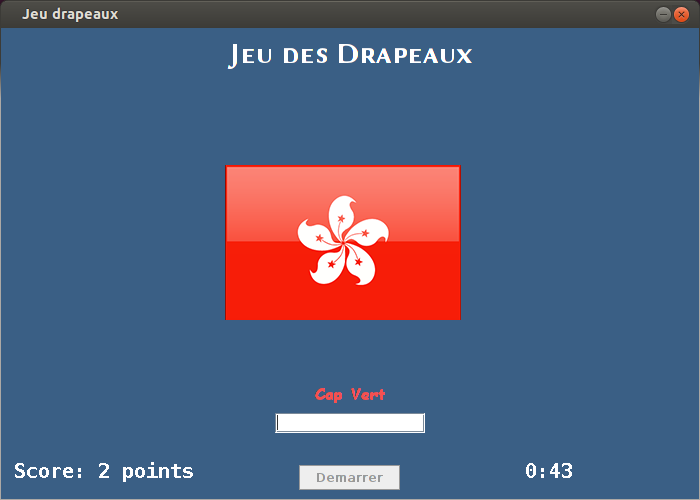
\includegraphics[scale=0.5]{capture2.png}\\
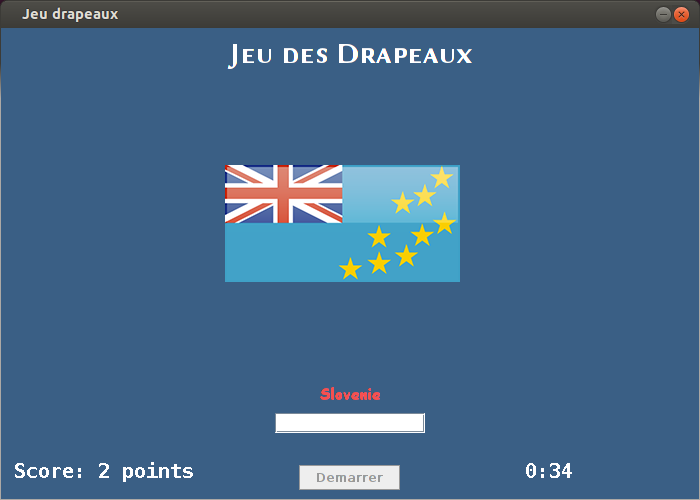
\includegraphics[scale=0.5]{capture3.png}\\
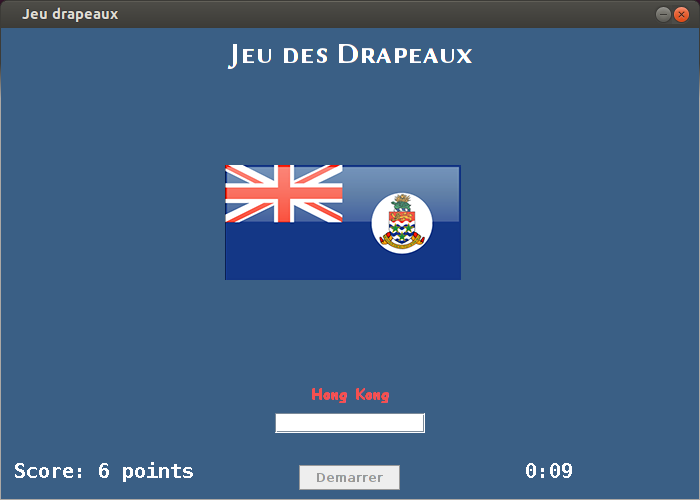
\includegraphics[scale=0.5]{capture4.png}\\
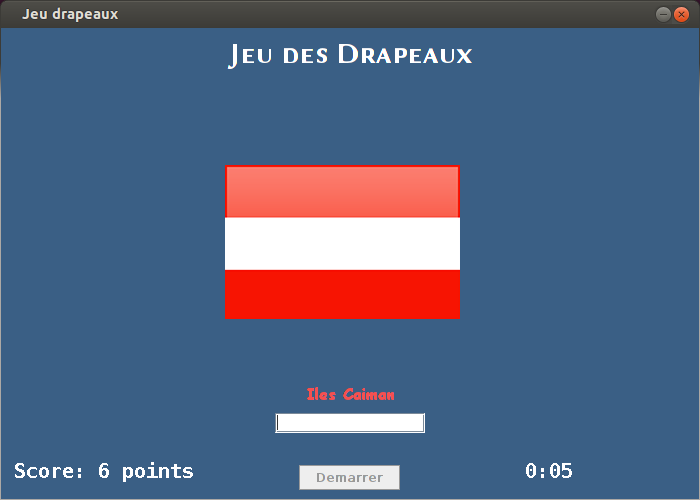
\includegraphics[scale=0.5]{capture5.png}\\
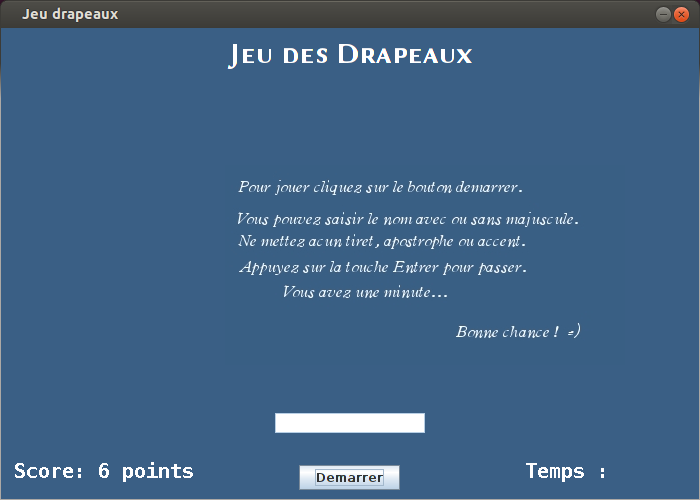
\includegraphics[scale=0.5]{capture6.png}
\end{center}

\newpage
\section*{Conclusion}
Pour conclure, on peut dire que ce projet nous aura permis d'acquérir une certaine aisance en JAVA. Il nous aura permis de mettre à l'épreuve les connaissances que nous avions déjà mais surtout de voir un peu plus loin. Les interfaces graphiques et les patterns nous étaient totalement inconnu avant de commencer ce projet, il nous aura donc beaucoup enrichi.

\end{document}
